%\chapter{Algebraic Concepts}
%\label{ch1}
%\thispagestyle{empty}
%\protected@edef\concepteq{%
%\[\conceptequiv\]
%}

\begin{wrapfigure}{r}{0.5\textwidth}
  \begin{center}
    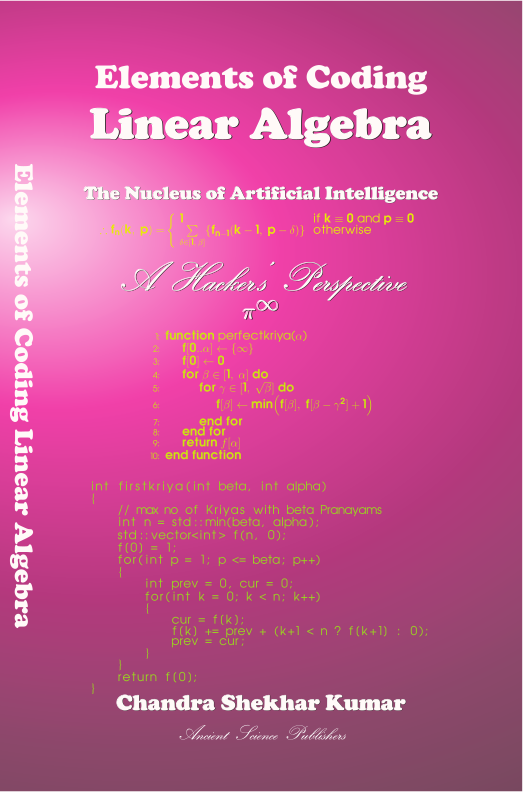
\includegraphics[width=0.5\textwidth]{codingla/cover}
  \end{center}
  %\caption{Front Cover}
\end{wrapfigure}

\underline{\textcolor{BurntOrange}{\textbf{Excerpt from the Chapter \Large \textcolor{Sepia}{Algebraic Concepts}}}}

\vspace{5mm}

\hspace{4mm}\hlt{\textbf{Concept} $\mathcal{C}$ is a predicate describing a set of syntactic and semantic requirements on related types ($<T_i>$) together with a collection of similar procedures $\left(f : T^i \rightarrow T^j\right)$ stated in terms of the properties, attributes and type functions $\left(F : \mathcal{C}^i \rightarrow \mathcal{C}^j \right)$ defined on the types.}
\begin{gather*}
\therefore \mathcal{C}\left(<T_i>\right) \conceptequiv \wedge <\Psi_j>
\end{gather*}
where $\conceptequiv$ stands for \hlt{is defined by} and the $\Psi_j$ represent independent clauses defining the concept.

\begin{lstlisting}
template<class T>
    concept integral = is_integral_v<T>;
\end{lstlisting}

\hlt{If a type $T$ fulfills all the requirements of a concept $\mathcal{C}$, then $T$ \textbf{models} $\mathcal{C}$}, i.e. $T \models \CC$.

\begin{nscenter}
int8\_t and uint8\_t $\models$ \concept{integral}.
\end{nscenter}

\hlt{Concept $\mathcal{C}^i$ is a \textbf{refinement} of concept $\mathcal{C}^j$ if it subsumes the latter, i.e. if $\mathcal{C}^i$ is true for a set of types, then $\mathcal{C}^j$ is also true for the same set.}

In other words, $\mathcal{C}^i$ \hlt{refines} $\mathcal{C}^j$ ($\mathcal{C}^i \refines \mathcal{C}^j$) by addition of more requirements to $\mathcal{C}^j$, i.e. $\mathcal{C}^j$ \hlt{weakens} $\mathcal{C}^i$ ($\mathcal{C}^j \weakens \mathcal{C}^i$). 

\begin{lstlisting}
template<class T>
    concept signed_integral = integral<T> && is_signed_v<T>;
\end{lstlisting}

\begin{nscenter}
\concept{signed\_integral} $\refines$ \concept{integral} \\
int8\_t $\models$ \concept{signed\_integral}  
\end{nscenter}

\begin{lstlisting}
template<class T>
concept unsigned_integral = integral<T> && !signed_integral<T>;
\end{lstlisting}

\begin{nscenter}
\concept{unsigned\_integral} $\refines$ \concept{integral} \\
uint8\_t $\models$ \concept{unsigned\_integral}  
\end{nscenter}




\begin{comment}

{\color{plotptcolor}
\vspace{1in}

\hrule
\vspace{1mm}
\hrule

\fancybreak{$\blacktriangle\blacktriangle\blacktriangle$}
\begin{hindi}
\centering \bfseries\large 
ॐ 
\end{hindi}
\fancybreak{$\blacktriangledown\blacktriangledown\blacktriangledown$}

\hrule
\vspace{1mm}
\hrule}
\end{comment}




